\documentclass[english,12pt,a4paper,pdftex]{article}
\usepackage[english]{babel}
\selectlanguage{english}
\usepackage[utf8]{inputenc}
\usepackage[elec,utf8]{aaltothesis}
\usepackage{graphicx}
\usepackage{url}
\usepackage[pdfpagemode=None,colorlinks=true,urlcolor=red,%
linkcolor=blue,citecolor=black,pdfstartview=FitH]{hyperref}
\usepackage{amsfonts,amssymb,amsbsy}

%% Vaakasuunnan mitat, äLä KOSKE!
\setlength{\hoffset}{-1in}
\setlength{\oddsidemargin}{35mm}
\setlength{\evensidemargin}{25mm}
\setlength{\textwidth}{15cm}
%% Pystysuunnan mitat, äLä KOSKE!
\setlength{\voffset}{-1in}
\setlength{\headsep}{7mm}
\setlength{\headheight}{1em}
\setlength{\topmargin}{25mm-\headheight-\headsep}
\setlength{\textheight}{23cm}

\newcommand{\publishedDate}{00.00.2014}

\begin{document}

\department{Department of Automation and Systems Technology}%
{Automaatio- ja systeemitekniikan laitos}
\professorship{Media Technology}{Viestintätekniikka}
\code{AS-75}

\univdegree{MSc}
\author{Marko Raatikka}

\thesistitle{LuminoTrace: a novel approach for identifying objects for the Web of Things}{}

\place{Espoo}

\date{\publishedDate{}}

\supervisor{Prof.\ Petri Vuorimaa}{Prof.\ Petri Vuorimaa}
\instructor{D.Sc.\ (Tech.) Jari Kleimola}{TkT Jari Kleimola}
\instructor{Prof.\ (Tech.) Jouni Paltakari}{Prof.\ Jouni Paltakari}

% \uselogo{aaltoRed|aaltoBlue|aaltoYellow|aaltoGray|aaltoGrayScale}{?|!|''}
\uselogo{aaltoRed}{''}

\makecoverpage

\keywords{LuminoTrace, JavaScript, hybrid, mobile, application, WWW, Web}
\begin{abstractpage}[english]
 % Your abstract in English. Try to keep the abstract short, approximately
 % 100 words should be enough. Abstract explains your research topic,
 % the methods you have used, and the results you obtained.


\end{abstractpage}

\newpage

%% Finnish abstract
\keywords{LuminoTrace, JavaScript, hybridi, mobiili, applikaatio, WWW, Web}
\begin{abstractpage}[finnish]
\end{abstractpage}

\mysection{Preface}


\vspace{1cm}
\noindent Otaniemi, \publishedDate{}\\

\vspace{0.15cm}
\noindent Marko Raatikka

\newpage

\thesistableofcontents
%% Symbols and abbreviations
\mysection{Symbols and abbreviations}
\subsection*{Symbols}

\begin{tabular}{ll}
%$|a_{ij}|^2$, $|a_i|^2$ & probability of two electrons having momenta
%    $\boldsymbol p_i$ and $\boldsymbol p_j$ ($\boldsymbol p_i$ for $|a_i|^2$) \\
%                 & at any given instant \\
$\mathbf{B}$  & magneettivuon tiheys  \\
$c$              & valon nopeus tyhjässä $\approx 3\times10^8$ [m/s]\\
%$p$              & magnitude of momentum \\
%$\boldsymbol p$, $\boldsymbol p_i$, $\boldsymbol p_i^{'}$  & momentum vector \\
%$p$              & magnitude of momentum \\
%$\boldsymbol p$, $\boldsymbol p_i$, $\boldsymbol p_i^{'}$  & momentum vector \\
%$\boldsymbol P$  &  \\
%$p_{\mathrm{F}}$ & Fermi momentum \\
$\omega_{\mathrm{D}}$    & Debye-taajuus \\
$\omega_{\mathrm{latt}}$ & hilan keskimääräinen fononitaajuus \\
$\uparrow$       & elektronin spinin suunta yläspäin\\
$\downarrow$     & elektronin spinin suunta alaspäin
\end{tabular}

\subsection*{Opetators}

\begin{tabular}{ll}
$\nabla \times \mathbf{A}$              & vektorin $\mathbf{A}$ roottori\\
$\displaystyle\frac{\mbox{d}}{\mbox{d} t}$ & derivaatta muuttujan $t$ suhteen\\
[3mm]
$\displaystyle\frac{\partial}{\partial t}$  & osittaisderivaatta muuttujan $t$ suhteen \\[3mm]
$\sum_i $                       & Summa indeksin $i$ yli\\
$\mathbf{A} \cdot \mathbf{B}$    & vektorien $\mathbf{A}$ ja $\mathbf{B}$ pistetulo
\end{tabular}

\subsection*{Abbreviations}

\begin{tabular}{ll}
AC         & vaihtovirta \\
APLAC      & an object-oriented analog circuit simulator and design tool \\
           & (originally Analysis Program for Linear Active Circuits) \\
BCS        & Bardeen-Cooper-Schrieffer \\ %% tavuviiva - nimien välissä
DC         & tasavirta \\
TEM        & transverse eletromagnetic
\end{tabular}

\cleardoublepage
\storeinipagenumber
\pagenumbering{arabic}
\setcounter{page}{1}


\section{Introduction}
\subsection{Research questions}

\thispagestyle{empty}
The focus of this thesis is the design and implementation of a scalable hybrid mobile application. The application will be developed as a part of the LuminoTrace project at Aalto CHEM for the purposes material verification. The functionality of the application can be briefly described as follows:

\begin{enumerate}
\item A user takes an image of a material with his/her mobile device
\item An algorithm analyzes the image and returns a unique digital fingerprint
\item The fingerprint is compared against a database of fingerprints
\item The user is notified whether or not a match was found.
\end{enumerate}

The verification is done by analyzing the spectrum of a special chemical compound embedded in the material. Both the underlying algorithm and the compound have already been developed as a part of the LuminoTrace project.

The implementation of the application can be divided into the following tasks:

\begin{itemize}
\item[--]Access and control built-in camera of the mobile device
\item[--]Port the code of the spectrum analysis algorithm to JavaScript
\item[--]Implement the UI
\item[--]Implement the back end infrastructure (cloud)
\end{itemize}

\begin{figure}[hbs]
\centering 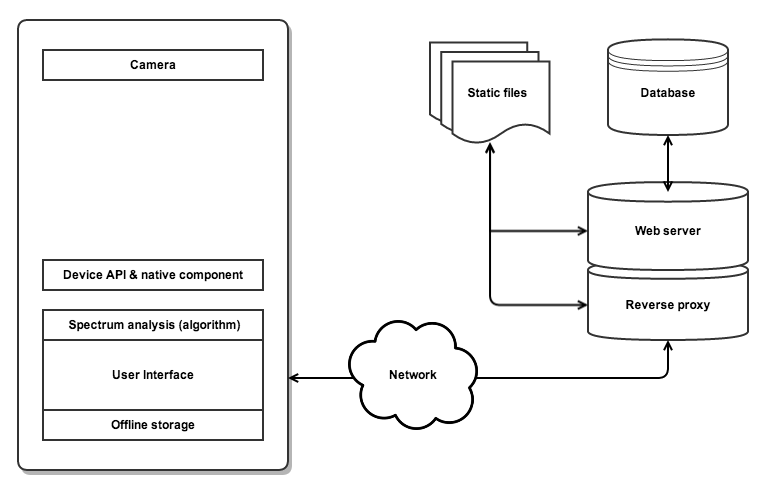
\includegraphics[width=13.25cm]{assets/diagram_0404}
\caption{A high-level overview of the structure of the application \label{diagram}}
\end{figure}

The functionality outlined above can be largely achieved by utilizing existing Web technologies and the W3C Device APIs. However, a more granular control over the camera (e.g. burst-mode, flash settings) will require a native component to be implemented for each target platform. The preliminary target platform will be Windows Phone (WP). To improve scalability the fingerprint will be computed on the client-side. This will require for the existing algorithm to be ported into JavaScript. Scalability can be further improved by offloading parts of the (fingerprint) database from the server to the user's device. Moreover, usability is improved as the application can function offline without the overhead of network latency. Hosting fingerprint data on the user's device might however have security implications: can the data be safely/efficiently encrypted on the user's device?

The underlying server back end will consist of a web server and a database to hold the fingerprint data. Optionally, a reverse proxy can be set up in front of the web server to allow static assets to be served to the client without hitting the web server. However, since the application will most likely not include many static assets (images, JS, CSS...) the benefit of this is somewhat minimal. The back end will be implemented using Node.js due to its convenience (author's previous experience and the possibility to re-use the ported spectrum algorithm both in the front and back end). The database will be implemented with MongoDB as it couples well with Node.js and has cross-platform support and an active community.

A high-level overview of the main components and interfaces of the application described above is given in Figure \ref{diagram}.

Hybrid apps are essentially small websites running in a browser shell in an app that have access to the native platform layer. Hybrid apps have many benefits over pure native apps, specifically in terms of platform support, speed of development, and access to 3rd party code.

% Johdanto selvittää samat asiat kuin tiivistelmä, mutta laveammin. Johdannossa kerrotaan yleensä seuraavat asiat

% \begin{itemize}
% \item[--]Tutkimuksen taustaa ja tutkimusaiheen yleisluonteinen esittely
% \item[--]Tutkimuksen tavoitteet
% \item[--]Pääkysymys ja osaongelmat
% \item[--]Tutkimuksen rajaus ja keskeiset käsitteet.
% \end{itemize}

% Lyhyiden opinnäytteiden johdannot ovat yleensä liian pitkiä, joten
% johdannon paisuttamista on vältettävä. Diplomityähän sopii johdanto,
% joka on 2--4 sivua. Kandidaatintyän johdannon on oltava diplomityän
% johdantoa lyhyempi. Sopivasti tiivistetty johdanto ei kaipaa alaotsikoita.




%% In a thesis, every section starts a new page, hence \clearpage
\clearpage

\section{Background}

Tässä osassa selvitetään, mitä tutkimuksen kohteena olevasta
aiheesta tiedetään entuudestaan. Selvityksen tulee kattaa
tasapainoisesti koko tutkimuskenttä.

How to connect objects to WoT
Object identification/verification
Web of Things (passive and active objects)

\subsection{Hybrid Applications}
\subsubsection{W3C Device APIs}
\subsubsection{Apache Cordova}

\subsection{Mobile Platforms}

\subsection{Web Workers}

\subsection{Offline Web Applications}

\subsection*{Structure}

Opinnäytteen rakenteen tulee olla hyvän tieteellisen
kirjoittamisen käytännän mukainen ja sisältää vähintään seuraavat
osat:

\begin{enumerate}
\item Nimiälehti
\item Tiivistelmä
\item Sisällysluettelo
\item Symboli- ja lyhenneluettelo
\item \label{a} Johdanto
%% Tässä alla on esimerkki lainausmerkkien käytästä. Suomalaisen tekstin
%% lainausmerkit eivät mene oikein latexissa (tai monissa muissakaan
%% julkaisujärjestelmissä) kun käytetään
%% "-merkkiä, koska latex käyttää amerikkalaista lainausmerkkien
%% tulostustapaa. Vaihtoehtona voi käyttää kulmalainausmerkkejä, jotka
%% myäs tulostuvat oikein.
\item  Aikaisempi tutkimus. Tyän luonteen niin vaatiessa otsikko voi olla myäs
        >>Teoreettinen tausta>>  tai näiden otsikoiden yhdistelmä.
\item Tutkimusaineisto ja -menetelmät %% yhdysmerkki - eli tavuviiva.
\item Tulokset
\item \label{o} Tarkastelu. Tyän luonteen niin vaatiessa otsikko voi
      olla myäs >>Johtopäätäkset>> tai >>Yhteenveto>>
      tai edellä mainittujen otsikoiden yhdistelmä.
\item Lähteet
\item Liitteet.
\end{enumerate}

Tiivistelmän ja symboli- sekä lyhenneluetteloiden
väliin voi sijoittaa halutessaan esipuheen.

Tyän osat \ref{a}-\ref{o} muodostavat \textit{tekstiosan.}  Tyän
yksittäisiä osia voidaan jakaa alaotsikoilla alaosiin, joita ei ole
yllä esitetty. Alaotsikoiden käyttäminen selventää parhaimmillaan
tekstiä, ja pahimmillaan sirpaloittaa sitä.  Sirpaloitumista voi estää
huolehtimalla siitä, että samalla sivulla ei esiinny useampaa
alaotsikkoa.  Tekstin jäsentelyssä on yleensä ongelmia, jos osassa on
vain yksi alaosa, tai kirjoittaja joutuu käyttämään useampaa kuin
kahta tasoa (osa ja alaosat): alaosien alaosat ovat harvoin tarpeen.
\subsection*{Sivut ja kirjaintyypit}

Opinnäytteen tulee olla kirjoitettu koneella tai
tekstinkäsittelyohjelmalla yksipuolisesti A4-kokoiselle paperille.
Kandidaatintyän tekstiosan sopiva pituus on noin 15--20 sivua ja
diplomityän noin 60 sivua. Tyätä ei ole syytä tarpeettomasti pidentää.

Opinnäytteen tekstiosan kirjaintyypin tulee olla antiikva eli
%% esimerkki pakkotavutuksesta; "serif-tyyppinen" on tavutuksen kannalta
%% hankala, joten pakkotavutetaan se.
serif\--tyyp\-pi\-nen ja lisäksi kursivoimaton, lihavoimaton sekä kooltaan 12
pistettä (kuten tässä esityksessä). Groteskeja eli \textsf{Sans
  serif}-tyyppisiä kirjaintyyppejä (kuten Helvetica tai Arial) ei saa
käyttää varsinaisessa tekstissä, mutta otsikoissa näitä voidaan
käyttää.  Otsikoissa voidaan käyttää kooltaan edellä mainittua
suurempaa kirjaintyyppiä sekä tyylikeinoja, kuten lihavointia tai
kursivointia.  Tekstissä samantasoisten otsikoiden on kuitenkin oltava
tyyliltään ja kirjainlajeiltaan yhteneväisiä.


\begin{table}[htb]
%% Taulukon teksti
\caption{Taulukoissa ja kuvissa kirjaintyypin voi valita
tarkoituksenmukaisesti, mutta kuva- ja taulukkoteksteissä tulee
käyttää samaa kirjaintyyppiä kuin varsinaisessa tekstissä.
Huomaa taulukon numeroinnin sijoittuminen taulukon yläpuolelle. \label{taulukko1}}
\begin{center}
\fbox{
\begin{tabular}{c|l|r}
\textbf{A} & 1 & $e^{j \omega t}$ \\ \hline
\textsf{B} & 2 & ${\mathfrak R}(c)$ \\ \hline
\texttt{C} & 3 & $ a \in \mathbb{A}$
\end{tabular}
}
\end{center}
\end{table}

Opinnäytteen vasen marginaali (sidonnan puoli) on
35~mm % tässä ~ muodostaa ns. yhdistävän välilyännin
ja oikea 25~mm. Ylämarginaali on 25~mm. Leipätekstin korkeus on
enimmillään 230mm. Tämän opinnäytepohjan marginaalien pitäisi olla
paperille tulostettuna oikein, mutta tulostimesta ja paperista
riippuen voi esiintyä yhden tai kahden millimetrin suuruisia eroja.
%% Jos käännät tämän tekstin pdflatex-komennolla ja tulostat sen katselu-
%% ohjelmasta, toteat todennäkäisesti em. mittojen poikkeavan enemmän
%% kuin 1-2 mm.
%% Tämä on seurausta pdf-tiedoston erilaisesta kirjaintyyppimäärityksestä.
%% Korkeatasoista painotyätä varten käytä vain latex-komentoa ja
%% tulosta postscript-muotoon käännetystä tiedostosta.
\subsection*{Placing}

Tekstiosan tekstissä käytetään kappaleiden erottamiseen sisennystä,
mutta ensimmäistä otsikon, väliotsikon tai muun katkon jälkeistä
kappaletta ei sisennetä. Jos kuva tai muu katko tulee kappaleiden
väliin, suositellaan katkon jälkeisen kappaleen sisentämistä.

Mikäli oikea reuna halutaan tasata, tulee käyttää tavutusta ja lisäksi
tarkistaa, ettei tekstiin jää lukemista häiritseviä pitkiä sanavälejä. Jos
käytät opinnäytteen tekemisessä \LaTeX-järjestelmää,
tämä asia hoituu automaattisest.

Opinnäytteen riviväli on 1, mikä on myäs tämän opinnäytepohjan käytäntä.
Kappaleiden tulee yleensä olla ainakin kolmen rivin pituisia, mutta
myäs liian pitkiä kappaleita tulee välttää.  Tässä opinnäytepohjassa
ei tekstin luonteen vuoksi voida täysin toteuttaa kappaleen pituutta koskevia
vaatimuksia.

Yksittäisiä, kappaleen päättäviä tai aloittavia rivejä sivun alussa
tai lopussa on vältettävä koko tyässä, myäs luetteloissa ja
liitteissä.

\subsection*{Numbering}

Opinnäytteen jokainen osa alkaa uudelta sivulta. Alaosa aloittaa uuden
sivun vain edellisen sivun täytyttyä.

Tyän osat numeroidaan siten, että johdanto on ensimmäinen numeroitava
osa. Osien numeroinnissa käytetään arabialaisia numeroita.

Nimiälehti, tiivistelmä, esipuhe, sisällysluettelo ja symboli- ja
lyhenneluettelo numeroidaan esipuheesta tai tämän puuttuessa
ensimmäiseltä luettelosivulta alkaen roomalaisin numeroin.

Sivunumerointi alkaa toiselta varsinaiselta tekstisivulta, ja
sivunumeroinnissa käytetään arabialaisia numeroita.

Lähdeluettelo alkaa uudelta sivulta. Lähdeluettelon sivunumerointi
jatkuu viimeisestä tekstisivusta.

Jokainen liite alkaa uudelta sivulta. Liitteiden sivunumerointi
jatkuu viimeisestä lähdeluettelon sivusta.

Sivunumero sijoitetaan sivun yläreunaan.

Matemaattiset kaavat numeroidaan arabialaisin
numeroin. Kaavanumerointi ei saa katketa osien välissä (eikä niin
tapahdukaan, jos käytät tätä opinnäytepohjaa). Kaikkia kaavoja ei tarvitse
numeroida, vaan kirjoittaja voi käyttää harkintaa numeroinnin
tarpeellisuudessa.  Liitteissä olevat kaavat numeroidaan siten, että
liitteen ajatellaan muodostavan numeroinnin kannalta itsenäisen ja
yhtenäisen kokonaisuuden. Kaavan numero sijoitetaan oikealle puolelle
alla olevan esimerkin mukaisesti
\begin{equation}
D(xy) = (Dx)y + x(Dy),  \hspace{3em} x,y \in \mathbb{A}.
\end{equation}
%% Kaavojen jälkeen ei yleensä laiteta sisennystä.
Kaikki kuvat ja taulukot numeroidaan erillisen juoksevan numeroinnin
mukaisesti kuten taulukosta \ref{taulukko1} ja kuvasta \ref{kuva1} käy
ilmi.  Liitteissä olevat kuvat ja taulukot numeroidaan siten, että
liitteen ajatellaan muodostavan numeroinnin kannalta itsenäisen ja
yhtenäisen kokonaisuuden. Liitteissä \ref{LiiteA} ja \ref{LiiteB} on
esimerkkejä kaavojen (kaavat \ref{liitekaava1}--\ref{liitekaava2} tai
kaavat \ref{liitekaava3}--\ref{liitekaava4}), kuvien (kuva
\ref{liitekuva}) ja taulukoiden (taulukko \ref{liitetaulukko})
numeroimisesta.  Liitteet numeroidaan suuraakkosin (esimerkiksi Liite
A, Liite B tai pelkästään A, B).

\begin{figure}[htb]
\centering 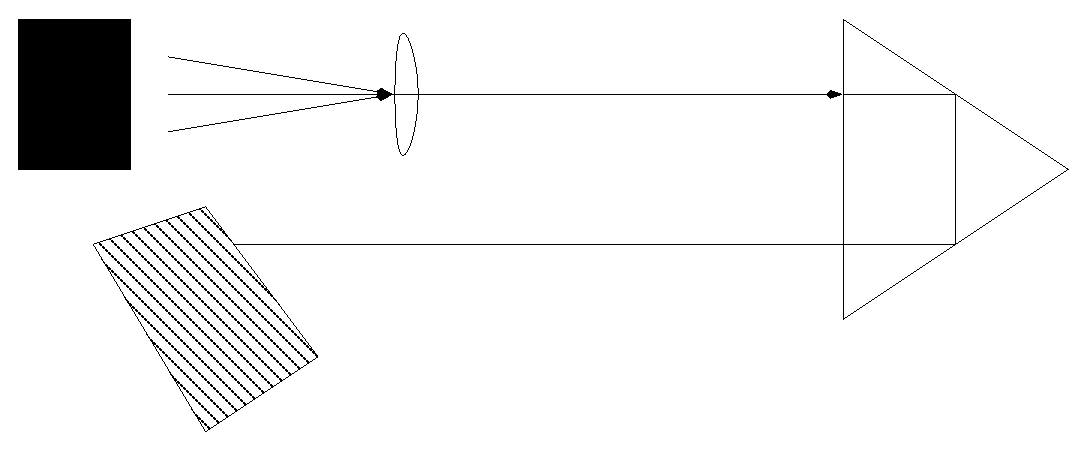
\includegraphics[height=5cm]{assets/kuva1}
\caption{Tämä on esimerkki numeroidusta kuvatekstistä. \label{kuva1}}
\end{figure}

\subsection*{Referencing}

Lähdeviittaukset tulee tehdä huolellisesti ja johdonmukaisesti
numeroviitejärjestelmän mukaisesti. Numeroviitteet järjestetään
lähdeluetteloon viittausjärjestykseen, mutta jos lähdeluettelo
on hyvin laaja (useita sivuja), järjestetään viitteet pääsanan
mukaiseen aakkosjärjestykseen. Alaviitejärjestelmää
\footnote{Myäskään alaviitteenä olevia kommentteja \underline{ei} suositella
käytettäviksi.} ei käytetä.

Viitteen sijoittelussa noudatetaan seuraavia sääntäjä:
Jos viite kohdistuu vain yhteen virkkeeseen tai virkkeen
osaan, viite \cite{Kauranen} sijoitetaan virkkeen sisään ennen virkettä
päättävää pistettä. Jos taas viite koskee tekstin useampaa
virkettä tai kokonaista kappaletta, sijoitetaan viite kappaleen loppuun
pisteen jälkeen. \cite{Kauranen}

\subsection*{References}

Lähdeluettelossa esiintyy tavallisesti seuraavassa esitettäviä
lähteitä, joista on numeroviitejärjestelmässä ilmoitettava
asianomaisessa kohdassa vaaditut tiedot.

%% Esimerkki korostamisesta. Lihavoinnin sijasta on tyylikkäämpää
%% ja luettavampaa käyttää kursiivia.
\textit{Kirjasta} ilmoitetaan seuraavat tiedot:

\begin{itemize}
\item[--]tekijät
\item[--]julkaisun nimi
\item[--]painos, jos useita
\item[--]kustannuspaikka
\item[--]julkaisija tai kustantaja
\item[--]julkaisuaika
\item[--]mahdollinen sarjamerkintä.
\end{itemize}

Viitteet \cite{Kauranen}--\cite{Koblitz} ovat esimerkkejä kirjan
esittämisestä lähdeluettelossa. Viite \cite[s.\ 83--124]{Koblitz} on
esimerkki lähdeluettelossa esiintyvän kirjan tiettyjen sivujen
esittämisestä tekstissä.

\textit{Artikkelista} kausijulkaisussa ilmoitetaan seuraavat tiedot:

\begin{itemize}

\item[--]tekijät
\item[--]artikkelin nimi
\item[--]kausijulkaisun nimi
\item[--]julkaisuvuosi
\item[--]kausijulkaisun volyymi tai ilmestymisvuosi
\item[--]kausijulkaisun numero
\item[--]sivut, joilla artikkeli on.
\end{itemize}

Viitteet \cite{bcs}--\cite{Deschamps} ovat esimerkkejä artikkelin
esittämisestä lähdeluettelossa.

\textit{Kokoomateoksen luvusta tai osasta} ilmoitetaan seuraavat tiedot:

\begin{itemize}
\item[--]luvun tai osan tekijät
\item[--]luvun tai osan nimi
\item[--]maininta >>Teoksessa>>
\item[--]koko teoksen toimittajat sekä maininta >>(toim.)>>
\item[--]koko teoksen tai konferenssin nimi
\item[--]konferenssiesitelmän kyseessä ollessa sen pitopaikka ja -aika
\item[--]painos, jos useita
\item[--]kustannuspaikka
\item[--]julkaisija tai kustantaja, jos aihetta tämän ilmoittamiseen on
\item[--]julkaisuaika
\item[--]sivut, joilla luku tai osa on
\item[--]mahdollinen sarjamerkintä.
\end{itemize}

Viitteet \cite{Sihvola}--\cite{Lindblom} ovat esimerkkejä
kokoomateoksen luvun tai osan esittämisestä lähdeluettelossa.

\textit{Opinnäytetyästä} ilmoitetaan seuraavat tiedot:

\begin{itemize}
\item[--]tekijä
\item[--]tyän nimi
\item[--]opinnäytetyän tyyppi
\item[--]oppilaitoksen nimi
\item[--]osaston, laitoksen tai ohjelman nimi
\item[--]oppilaitoksen sijaintipaikka
\item[--]vuosiluku.
\end{itemize}

Viitteet \cite{Miinusmaa}--\cite{Lonnqvist} ovat esimerkkejä
opinnäytteen esittämisestä lähdeluettelossa.

\textit{Standardista} ilmoitetaan seuraavat tiedot:

\begin{itemize}
\item[--]standardin tunnus ja numero
\item[--]standardin nimi
\item[--]painos, mikäli ei ole ensimmäinen
\item[--]julkaisupaikka
\item[--]julkaisija
\item[--]julkaisuvuosi
\item[--]sivumäärä.
\end{itemize}
Viite \cite{sfs} on esimerkki standardin esittämisestä opinnäytteen
lähdeluettelossa.

\textit{Haastattelusta} ilmoitetaan seuraavat tiedot:

\begin{itemize}
\item[--]haastatellun henkilän nimi
\item[--]haastatellun henkilän arvo tai asema
\item[--]haastatellun henkilän edustama organisaatio
\item[--]organisaation osoite
\item[--]maininta siitä, että kyseessä on haastattelu ja haastattelun
päivämäärä.
\end{itemize}

Viite \cite{haastattelu} on esimerkki
haastattelun esittämisestä lähdeluettelossa.

Osa sähkäisessä muodossa olevista artikkeleista on saatavissa myäs
painettuina. \textit{Vain verkosta saatavissa olevasta artikkelista} esitetään
seuraavat tiedot:

\begin{itemize}
\item[--]tekijät
\item[--]artikkelin nimi
\item[--]kausijulkaisun nimi
\item[--]viestintyyppi
\item[--]laitos tai volyymi
\item[--]kausijulkaisun yksittäistä osaa koskeva merkintä tai numero
\item[--]julkaisuvuosi tai maininta >>Päivitetty>> ja päivitysaika
\item[--]maininta >>Viitattu>> ja viittaamisen ajankohta
\item[--]maininta >>Saatavissa>> ja URL tai
        maininta >>DOI>> ja DOI-numero (DOI=Digital Object Identifier).
\end{itemize}

Viitteet \cite{Ribeiro}--\cite{kone} ovat esimerkkejä sähkäisessä
muodossa olevan artikkelin esittämisestä opinnäytteen
lähdeluettelossa.  Viitteet \cite{Ribeiro} ja \cite{Stieber} ovat
saatavissa sekä painettuna että verkosta, joten viitteiden esitystapa
mukailee painetun artikkelin viitteen esitystapaa, mutta sen lisäksi
kerrotaan julkaisun olevan verkkolehti ja lehden olevan saatavissa
myäs painettuna.  Viite \cite{kone} on saatavissa vain verkosta ja
siitä esitetään yllä vaaditut tiedot.

Valitettavasti sähkäisessä muodosssa olevasta artikkelista ei ole aina
saatavissa lai\-tos-, volyymi- tai numerotietoja.

\textit{Sähkäisessä muodossa olevasta opinnäytetyästä} ilmoitetaan
seuraavat tiedot:

\begin{itemize}
\item[--]tekijä
\item[--]tyän nimi
\item[--]viestintyyppi
\item[--]opinnäytetyän tyyppi
\item[--]oppilaitoksen nimi
\item[--]osaston, laitoksen tai ohjelman nimi
\item[--]oppilaitoksen sijaintipaikka
\item[--]vuosiluku
\item[--]viittamisen ajankohta
\item[--]maininta >>Saatavissa>> ja URL tai
        maininta >>DOI>> ja DOI-numero.
\end{itemize}

Viite \cite{Adida} on esimerkki sähkäisessä muodossa olevan
opinnäytteen esittämisestä lähdeluettelossa.

Viite \cite{viittaaminen} on esimerkki itsenäisen kirjoituksen sisältävästä
verkkosivusta. Tällainen lähde on rinnastettavissa erillisteokseen.
\textit{Verkkosivusta} esitetään tiedot:

\begin{itemize}
\item[--] tekijät
\item[--] otsikko
\item[--] maininta >>Päivitetty>> ja päivitysaika
\item[--] maininta >>Viitattu>> ja viittaamisen ajankohta
\item[--] Maininta >>Saatavissa>> ja URL.
\end{itemize}

Joskus verkkosivun kirjoitus on jaettu useammalle sivulle, jolloin
lähdeluetteloon kirjataan vain sellainen verkko-osoite, joka koskee
koko kirjoitusta tai sen etusivua, ellei sitten
todella tarkoiteta kirjoituksen yksittäistä sivua.

\subsection*{Other notes on referencing}

%% Muutos vanhoihin ohjeisiin koskien kieltä.
Lähdeluettelossa tyän ja julkaisun nimi kirjoitetaan alkuperäisessä
muodossaan. Julkaisijan kotipaikka kirjoitetaan alkukielisessä
muodossaan.

Viittamista koskevassa suomalaisessa standardissa
SFS 5342 \cite{sfs} vaaditaan julkaisuista ilmoitettavaksi myäs ISBN- tai
ISSN-numerot, mutta näissä opinnäyteohjeissa ei ISBN- ja
ISSN-numeroita vaadita.

\clearpage

\section{Design and implementation}

Tässä osassa kuvataan käytetty tutkimusaineisto ja
tutkimuksen metodologiset valinnat, sekä
kerrotaan tutkimuksen toteutustapa ja käytetyt menetelmät.

\subsection{Requirements}

\subsection{Development environment}

\subsection{Client-side architecture}

\subsubsection{Camera setup}

\subsubsection{Device interface}

\subsubsection{User Interface}

\subsection{Server-side architecture}

\clearpage

\clearpage

\section{Evaluation and discussion}
\subsection{Offline performance}
\subsection{Security considerations}

Tässä osassa esitetään tulokset ja vastataan tutkielman alussa
esitettyihin tutkimuskysymyksiin. Tieteellisen kirjoitelman
arvo mitataan tässä osassa esitettyjen tulosten perusteella.

%% Huomaa seuraavassa kappaleessa lainausmerkkien ulkopuolella piste,
%% koska piste ei lopeta lainattua tekstinpätkää.
%% Jos lainattu tekstinpätkä loppuu välimerkkiin, tulee välimerkki
%% lainausmerkkien sisälle:
%% "Et tu, Brute?" sanoi Caesar kuollessaan.
Tutkimustuloksien merkitystä on aina syytä arvioida ja tarkastella
kriittisesti.  Joskus tarkastelu voi olla tässä osassa, mutta se
voidaan myäs jättää viimeiseen osaan, jolloin viimeisen osan nimeksi
tulee >>Tarkastelu>>. Tutkimustulosten merkitystä voi arvioida myäs
>>Johtopäätäkset>>-otsikon alla viimeisessä osassa.

Tässä osassa on syytä myäs arvioida tutkimustulosten luotettavuutta.
Jos tutkimustulosten merkitystä arvioidaan >>Tarkastelu>>-osassa,
voi luotettavuuden arviointi olla myäs siellä.

\clearpage

\section{Conclusions}

Opinnäytteen tekijä vastaa siitä, että opinnäyte on tässä dokumentissa
ja opinnäytteen tekemistä käsittelevillä luennoilla sekä
harjoituksissa annettujen ohjeiden mukainen muotoseikoiltaan,
rakenteeltaan ja ulkoasultaan.



\clearpage


\phantomsection
\addcontentsline{toc}{section}{References}
\begin{thebibliography}{99}

%% Alla pilkun jälkeen on pakotettu oikea väli \<välilyänti>-merkeillä.
\bibitem{Kauranen} Kauranen,\ I., Mustakallio,\ M. ja Palmgren,\ V.
  \textit{Tutkimusraportin kirjoittamisen opas opinnäytetyän
    tekijäille.}  Espoo, Teknillinen korkeakoulu, 2006.

\bibitem{Itkonen} Itkonen,\ M. \textit{Typografian käsikirja.} 3.\
  painos.  Helsinki, RPS-yhtiät, 2007.

\bibitem{Koblitz} Koblitz,\ N. \textit{A Course in Number Theory and
    Cryptography. Graduate Texts in Mathematics 114.}  2.\ painos. New
  York, Springer, 1994.

%% Kun on useampi nimikirjain, jokaisen nimikirjaimen väliin
%% kuuluu välilyänti. Oikea välin määrä on saatu \<välilyännillä>
\bibitem{bcs} Bardeen,\ J., Cooper,\ L.\ N. ja Schrieffer,\ J.\ R.
  Theory of Superconductivity. \textit{Physical Review,} 1957, vol.\
  108, nro~5, s.\ 1175--1204.

\bibitem{Deschamps} Deschamps,\ G.\ A. Electromagnetics and
  Differential Forms. \textit{Proceedings of the IEEE,} 1981, vol.\
  69, nro~6, s.\ 676--696.

%% Alla esimerkki englanninkielisen tavuttamisen pakottamisesta.
%% Oletusarvoisesti käytetään suomalaista tavutusta, mutta viitteissä
%% esiintyy usein muunkielisiä lauseita, jotka tulevat siten tavutetuksi
%% suomen kielen sääntäjen mukaan. Tämän voi korjata \foreignlanguage-
%% komennolla, jonka ensimmäinen parametri on vieraan kielen nimi ja toinen
%% on vieraalla kielellä tavutettava teksti.
\bibitem{Sihvola} Sihvola,\ A.\ et al.
  \foreignlanguage{english}{Interpretation of measurements of helix
and bihelix superchiral structures.}  Teoksessa: Jacob,\ A.\ F. ja
  Reinert,\ J. (toim.) \textit{Bianisotropics '98 7th International
    Conference on Complex Media.}  Braunschweig, 3.--6.6.1998.
  Braunscweig, Technische Universität Braunschweig, 1998, s.\
  317--320.

%% Alla on suomalainen yhdistelmäsukunimi. Sen nimien välissä
%% käytetään yhdysmerkkiä l. tavuviivaa, kirjoitetaan -.
\bibitem{Lindblom} Lindblom-Ylänne,\ S. ja Wager,\ M.  Tieteellisten
  opinnäytetäiden ohjaaminen. Teoksessa: Lindblom-Ylänne,\ S. ja
  Nevgi,\ A. (toim.) \textit{Yliopisto- ja korkeakouluopettajan
    käsikirja.}  Helsinki, WSOY, 2004, s.\ 314--325.

\bibitem{Miinusmaa} Miinusmaa,\ H. Neliskulmaisen reiän poraamisesta
  kolmikulmaisella poralla. Diplomityä, Teknillinen korkeakoulu,
  konetekniikan osasto, Espoo, 1977.

%% Tässä taas pakotettu englanninkielinen tavutus.
%% Pedanttinen kirjoittaja pakottaa tietysti jokaiseen englanninkieliseen
%% lauseeseen englannin tavutuksen, mutta tässä esityksessä ei näin ole
%% tehty selvyyden ja lähdekoodin luettavuuden takia.
\bibitem{Loh} Loh,\ N.\ C. High-Resolution Micromachined
  Interferometric Accelerometer. Master's Thesis, Massachusetts
  Institute of Technology, Cambridge,
  \foreignlanguage{english}{Massachusetts,} 1992.

\bibitem{Lonnqvist} Lännqvist,\ A.
  \foreignlanguage{english}{Applications of hologram-based compact
    range: antenna radiation pattern, radar cross section, and
    absorber reflectivity measurements.} Väitäskirja, Teknillinen
  korkeakoulu, sähkä- ja tietoliikennetekniikan osasto, 2006.

\bibitem{sfs} SFS 5342. Kirjallisuusviitteiden laatiminen. 2.\ painos.
  Helsinki, Suomen standardisoimisliitto, 2004. 20~s.

\bibitem{haastattelu} Palmgren,\ V. Suunnittelija. Teknillinen
  korkeakoulu, kirjasto. Otaniementie 9, 02150 Espoo. Haastattelu
  15.1.2007.

\bibitem{Ribeiro} Ribeiro,\ C.\ B., Ollila,\ E. ja Koivunen,\ V.
  \foreignlanguage{english}{Stochastic Maximum-Likelihood Method for
    MIMO Propagation Parameter Estimation.} \textit{IEEE Transactions
    on Signal Processing,} verkkolehti, vol.\ 55, nro~1, s.\ 46--55.
  Viitattu 19.1.2007. Lehti ilmestyy myäs painettuna. DOI:
  10.1109/TSP.2006.882057.

\bibitem{Stieber} Stieber,\ T. GnuPG Hacks. \textit{Linux Journal,}
  verkkolehti, 2006, maaliskuu, nro~143. Viitattu 19.1.2007. Lehti
  ilmestyy myäs painettuna. Saatavissa:
  \url{http://www.linuxjournal.com/article/8732.}

\bibitem{kone} Pohjois-Koivisto,\ T. Voiko kone tulevaisuudessa arvata
  tahtosi?  \textit{Apropos,} verkkolehti, helmikuu, nro~1, 2005.
  Viitattu 19.1.2007.  Saatavissa:
  \url{http://www.apropos.fi/1-2005/prima.php.}

\bibitem{Adida} Adida,\ B.  Advances in Cryptographic Voting Systems.
  Verkkodokumentti. Ph.D.\ Thesis, Massachusetts Institute of
  Technology, Cambridge, \foreignlanguage{english}{Massachusetts,}
  2006. Viitattu 19.1.2007.  Saatavissa:
  \url{http://crypto.csail.mit.edu/~cis/theses/adida-phd.pdf.}

\bibitem{viittaaminen} Kilpeläinen,\ P. WWW-lähteisiin viittaaminen
  tutkielmatekstissä. Verkkodokumentti. Päivitetty 26.11.2001.
  Viitattu 19.1.2007. Saatavissa:
  \url{http://www.cs.uku.fi/~kilpelai/wwwlahteet.html.}

\end{thebibliography}

\clearpage

% \appendix
% \phantomsection
% \addcontentsline{toc}{section}{Appendices}

% \section{\label{LiiteA}}
%% Liitteiden kaavat, taulukot ja kuvat numeroidaan omana kokonaisuutenaan

\renewcommand{\theequation}{A\arabic{equation}}
\setcounter{equation}{0}
\renewcommand{\thefigure}{A\arabic{figure}}
\setcounter{figure}{0}
\renewcommand{\thetable}{A\arabic{table}}
\setcounter{table}{0}

Liitteet eivät ole opinnäytteen kannalta välttämättämiä ja
opinnäytteen tekijän on
kirjoittamaan ryhtyessään hyvä ajatella pärjäävänsä ilman liitteitä.
Kokemattomat kirjoittajat, jotka ovat huolissaan
tekstiosan pituudesta, paisuttavat turhan
helposti liitteitä pitääkseen tekstiosan pituuden annetuissa rajoissa.
Tällä tavalla ei synny hyvää opinnäytettä.

Liite on itsenäinen kokonaisuus, vaikka se täydentääkin tekstiosaa.
Liite ei siten ole pelkkä listaus, kuva tai taulukko, vaan
liitteessä selitetään aina sisällän laatu ja tarkoitus.

Liitteeseen voi laittaa esimerkiksi listauksia. Alla on
listausesimerkki tämän liitteen luomisesta.

%% Verbatim-ympäristä ei muotoile tai tavuta tekstiä. Fontti on monospace.
%% Verbatim-ympäristän sisällä annettuja komentoja ei LaTeX käsittele.
%% Vasta \end{verbatim}-komennon jälkeen jatketaan käsittelyä.
\begin{verbatim}
	\clearpage
	\appendix
	\addcontentsline{toc}{section}{Liite A}
	\section*{Liite A}
	...
	\thispagestyle{empty}
	...
	tekstiä
	...
	\clearpage
\end{verbatim}

Kaavojen numerointi muodostaa liitteissä oman kokonaisuutensa:
\begin{eqnarray}
d \wedge A  &=& F, \label{liitekaava1}\\
d \wedge F  &=& 0. \label{liitekaava2}
\end{eqnarray}


\clearpage
% \section{Toinen esimerkki liitteestä\label{LiiteB}}

%% Equations, tables and figures have their own numbering in Appendices
\renewcommand{\theequation}{B\arabic{equation}}
\setcounter{equation}{0}
\renewcommand{\thefigure}{B\arabic{figure}}
\setcounter{figure}{0}
\renewcommand{\thetable}{B\arabic{table}}
\setcounter{table}{0}

Liitteissä voi myäs olla kuvia, jotka
eivät sovi leipätekstin joukkoon:
%% Ympäristän figure parametrit htb pakottavat
%% kuvan tähän, eikä LaTeX yritä siirrellä niitä
%% hyväksi katsomaansa paikkaan.
%% Ympäristää center voi käyttää \centering-
%% komennon sijaan
%%
%% Example of a figure, note the use of htb parameters which force
%% the figure to be inserted here
\begin{figure}[htb]
\begin{center}
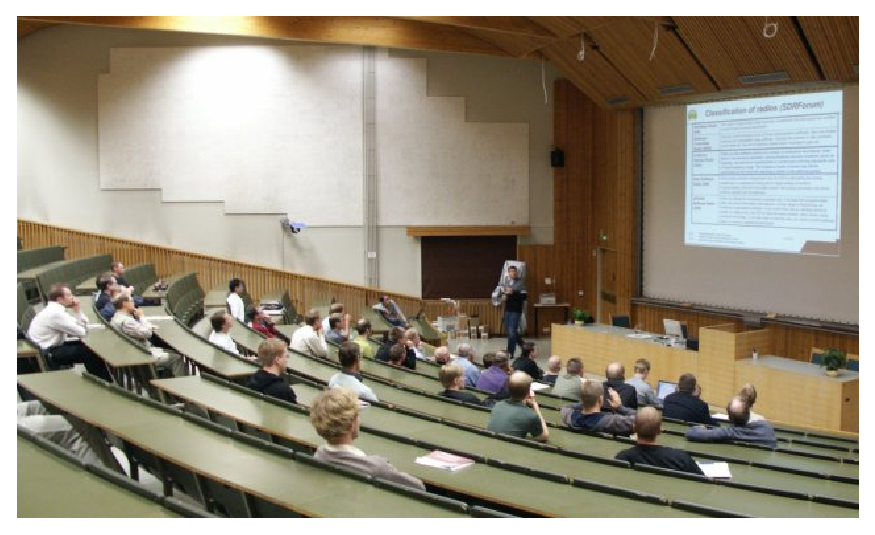
\includegraphics[height=8cm]{assets/kuva2}
\end{center}
\caption{Kuvateksti, jossa on liitteen numerointi \label{liitekuva}}
\end{figure}
%%
Liitteiden taulukoiden numerointi on kuvien ja kaavojen kaltainen:
\begin{table}[htb]
\caption{Taulukon kuvateksti. \label{liitetaulukko}}
\begin{center}
\fbox{
\begin{tabular}{lp{0.5\linewidth}}
9.00--9.55  & Käytettävyystestauksen tiedotustilaisuus (osanottajat
ovat saaneet sähkäpostitse valmistautumistehtävät, joten tiedotustilaisuus
voidaan pitää lyhyenä).\\
9.55--10.00 & Testausalueelle siirtyminen
\end{tabular}}
\end{center}
\end{table}
Kaavojen numerointi muodostaa liitteissä oman kokonaisuutensa:
\begin{eqnarray}
T_{ik} &=& -p g_{ik} + w u_i u_k + \tau_{ik},  \label{liitekaava3} \\
n_i    &=& n u_i + v_i.                        \label{liitekaava4}
\end{eqnarray}

\end{document}
